 \thispagestyle{gocconone}
\pagestyle{gocco}
\everymath{\color{gocco}}
\graphicspath{{../gocco/pic/}}
\blfootnote{$^1${\color[named]{gocco}Trung tâm Quy hoạch và Điều tra tài nguyên -- môi trường biển khu vực phía Nam.}}
\begingroup
\AddToShipoutPicture*{\put(0,616){\includegraphics[width=19.3cm]{../bannergocco}}}
\AddToShipoutPicture*{\put(164,554){\includegraphics[scale=1]{../tieude.pdf}}} 
\centering
\endgroup

\vspace*{150pt}
\begin{multicols}{2}
	Trên bàn cờ rộng lớn, có một quân cờ có khả năng tung hoành trên các nẻo đường ngang dọc, có cách ăn quân rất đặc biệt, bằng cách nhảy qua $1$ quân cờ khác. Loại binh chủng này sở hữu khả năng kiểm soát và khống chế tầm xa vô cùng hiệu quả, luôn sẵn sàng phục kích, chỉ cần chờ đợi có một ngòi nổ là có thể bắn phá trận địa của kẻ thù. Dù cho Tướng giặc có ẩn náu trong thâm cung bí hiểm với nhiều lớp bảo vệ, có lực lượng phòng vệ canh\linebreak gác cẩn mật, khi các quân khác khó lòng tiếp cận, nó vẫn có thể nã đạn cầu vồng để tiêu diệt. Trong nhiều tình huống, nó được kéo hẳn về Cửu cung mình, phối hợp cùng Sỹ, Tượng để ra đòn công sát.  Vâng, khi nhắc đến ``pháo", người ta thường hình dung đến loại vũ khí mạnh mẽ, thường được dùng để tiêu diệt các mục tiêu khó tiếp cận. Nhưng không, chúng ta chỉ đang nhắc tới SỰ LỢI HẠI của quân PHÁO trên bàn cờ mà thôi!  
	\vskip 0.05cm
	Tuy nhiên, có một điều thú vị ở đây là, Cờ Tướng thời cổ đại không có quân Pháo. Đây cũng là quân cờ có lịch sử ra đời muộn nhất trên bàn cờ Tướng. Các nhà nghiên cứu đều nhất trí rằng nó được được bổ sung từ thời nhà Đường. Ban đầu, từ Pháo (砲) trong chữ Hán được viết với bộ ``thạch", nghĩa là đá. Cho đến đời nhà Tống, khi loại pháo mới mang thuốc nổ được phát minh thì từ Pháo (炮) được viết với bộ ``hỏa"... Và kể từ khi Pháo xuất hiện, bàn Cờ Tướng trở nên cực kỳ sôi động, khói lửa mịt mù từ đầu tới cuối trận với những đòn thế vô cùng hiểm hóc. Có thể nói rằng, $2$ quân Pháo đã nâng Cờ Tướng lên một tầm cao hoàn toàn mới, khiến cho cờ Tướng trở nên cực kỳ hấp dẫn và độc đáo hơn nhiều. Nhờ có Pháo, hệ thống khai cuộc từ đó ngày càng phát triển với vô vàn trận hình liên quan, trong đó có những thế trận đã nên kinh điển theo thời gian, và được các kỳ thủ áp dụng rất nhiều trong \linebreak thực chiến. 
	\vskip 0.05cm
	Để biết thêm Pháo có sức mạnh như thế nào, chúng ta cùng nhau xem xét các ví dụ cụ thể dưới đây:
	\begin{figure}[H]
		\vspace*{-5pt}
		\centering
		\captionsetup{labelformat= empty, justification=centering}
		\includegraphics[width= 0.3\textwidth]{2}
		\caption{\small\textit{\color{gocco}Hình $1$.}}
		\vspace*{-10pt}
	\end{figure}
	$1.$ Đây là hình cờ tàn cơ bản, thoạt nhìn qua, có thể quân Pháo bị coi là vô hại vì không có ngòi để khoan phá. Nhưng  không, bên Đỏ đã biết cách vận dụng Pháp khéo léo để đi tới chiến thắng như sau: 
	\vskip 0.05cm
	$\pmb{1)}$	P$2-5$ $(*)$ X$5-9$\quad $\pmb{2)}$ X$6/6$ Tg$5/1$\quad $\pmb{3)}$ X6$-5$ Tg$5-6$\quad $\pmb{4)}$ P$5-3$ X$9-6$ $(**)$\quad $\pmb{5)}$ Tg$6-5$ X$6.1$\quad $\pmb{6)}$ X$5.6$ Tg$6/1$\quad $\pmb{7)}$ X$5.1$ Tg$6.1$\quad $\pmb{8)}$ P$3-4$ $(***)$ X$6-9$ \quad$\pmb{9)}$ X$5/7$ $(1-0)$
	\vskip 0.05cm
	$(*)$ \textit{Nước đi chuẩn xác và đầy uy lực, dùng chính quân Tướng đối phương làm ngòi cho Pháo, buộc Xe Đen phải rời đi khỏi trục lộ quan trọng.}
	\vskip 0.05cm
	$(**)$ \textit{Sau khi đuổi Xe đen, Đỏ lập tức đưa Xe chiếm lấy trung lộ, Đen lại phải lật đật đưa xe vào giữ mặt để tránh đòn chiếu bí.}
	\vskip 0.05cm
	$(***)$ Dựa vào mặt Tướng, Đỏ liên tục tấn Xe áp sát để Pháo tiếp tục bình vào tróc nã Xe đối phương, Đen dù nhìn thấy nước sát nhưng vẫn phải chấp nhận thất bại.
	\begin{figure}[H]
		\vspace*{-5pt}
		\centering
		\captionsetup{labelformat= empty, justification=centering}
		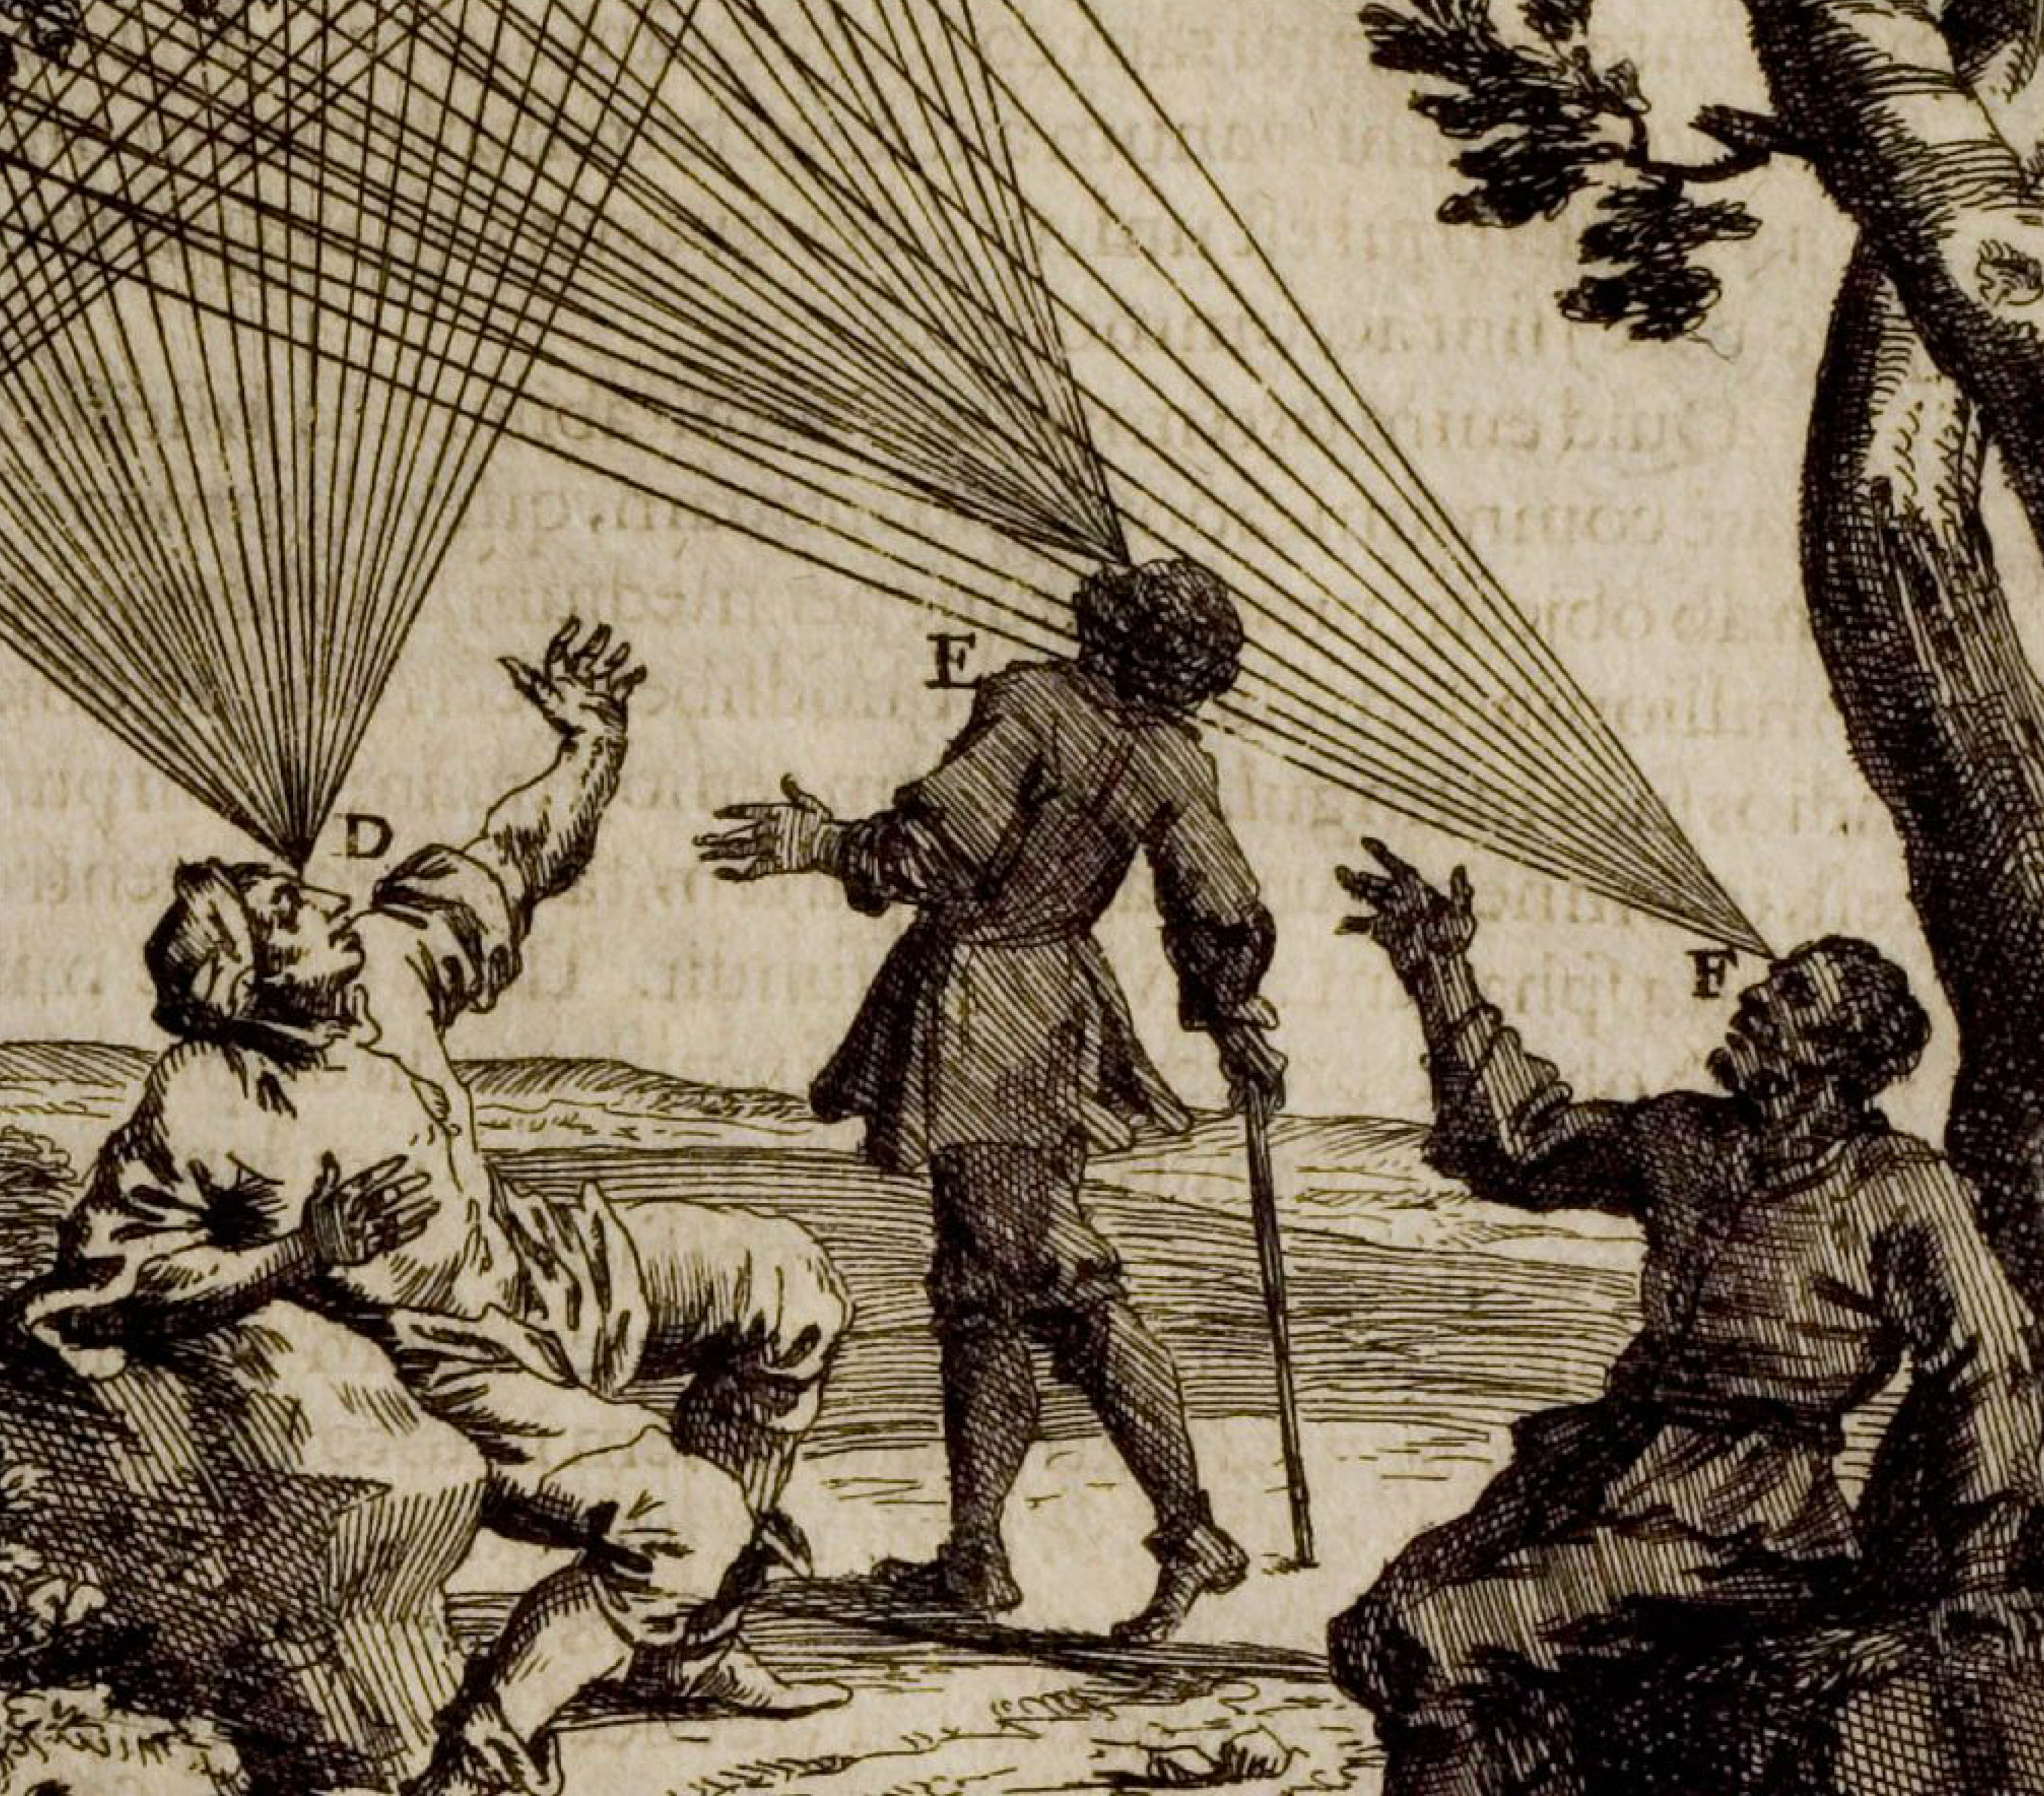
\includegraphics[width= 0.3\textwidth]{1}
		\caption{\small\textit{\color{gocco}Hình $2$.}}
		\vspace*{-10pt}
	\end{figure}
	$2.$ Hình $2$, bên Đen còn Mã, song Sĩ, $2$ chốt luôn chực chờ tiến vào cửu cung tạo sát. Nhưng bên Đỏ có quân Pháo vô cùng cơ động và được quyền đi trước. Đỏ đi:
	\vskip 0.05cm
	$\pmb{1)}$ C$3.1$ Tg$6-5$ $(*)$\quad  $\pmb{2)}$ P$9.1$ M$4/3$\quad $\pmb{3)}$ P$9/5$ M$3.4$\quad $\pmb{4)}$ P$9-1$ $(**)$ M$4.5$\quad $\pmb{5)}$ P$1-5$ C$8-7$ \quad $\pmb{6)}$ Tg$5-4$ $(***)$ $(1-0)$
	\vskip 0.05cm
	$(*)$ \textit{Chốt Đỏ ngang nhiên tiến xuống hàng đáy uy hiếp, Tướng đen không còn cách nào khác phải bình vào lộ $5$ để ẩn náu.}
	\vskip 0.05cm
	$(**)$ \textit{Liên tục là những nước điều Pháo rất \linebreak linh hoạt và có ý đồ của Đỏ, buộc Đen phải di chuyển Mã theo để phòng thủ hết sức vất vả.}
	\vskip 0.05cm
	$(***)$ \textit{Cuối cùng, đỏ bình Pháo vào trung lộ, khiến cho Tướng, Mã, song Sỹ của Đen kẹt cứng. Chỉ cần bình Tướng là cục thế được định đoạt, Đen chắc chắn thua cuộc.} 
	\begin{figure}[H]
		\vspace*{-5pt}
		\centering
		\captionsetup{labelformat= empty, justification=centering}
		\includegraphics[width= 0.3\textwidth]{3}
		\caption{\small\textit{\color{gocco}Hình $3$.}}
		\vspace*{-10pt}
	\end{figure}
	$3.$ Hình $3$, bên Đen đang có cơ hội lớn để \linebreak giành thắng lợi, khi chỉ cần đi X$7.7$ là chiếu bí. Và Đỏ không thể để điều đó xảy ra một cách dễ dàng, Đỏ đối phó như sau:
	\vskip 0.05cm
	$\pmb{1)}$	X$2-4$ X$7-6$ $(*)$\quad $\pmb{2)}$ P$8-4$ X$6-7$\quad $\pmb{3)}$ P$4-2$ X$7-6$\quad $\pmb{4)}$ P$9-4$ X$6-7$\quad $\pmb{5)}$ P$4-1$ X$7-6$ $(**)$\quad $\pmb{6)}$ P$1.5$ T$7.9$\quad $\pmb{7)}$ M$3/5$ Tg$6/1$ $(***)$\quad $\pmb{8)}$ $M5.6$ Tg$6.1$\quad $\pmb{9)}$ P$2-5$ $(1-0)$
	\vskip 0.05cm
	$(*)$ Đỏ đưa Xe chiếu Tướng chiếm trục lộ trọng yếu, buộc Đen phải dùng Xe che chắn. Đây cũng là thao tác cần thiết nhằm tạo điều kiện cho song Pháo Đỏ dễ dàng hoạt động.
	\vskip 0.05cm
	$(**)$ Lợi dụng Xe Đen làm ngòi, chỉ trong vòng $4$ nước, Đỏ đã đưa cặp Pháo từ cánh trái sang cánh phải một cách tài tình nhưng vẫn giữ được nước tiên, Đen chỉ có thể bình Xe tránh nước chiếu một cách thụ động.
	\vskip 0.05cm
	$(***)$ Đỏ tiếp tục cắm Pháo uy hiếp tuyến đáy của Đen làm cho đôi Tượng mất liên kết, tạo điều kiện cho Mã thoái về bắt Tượng ở lộ $5$ để uy hiếp Tướng. Thế trận sụp đổ, Đen đành chấp nhận thất bại.
	\vskip 0.05cm
	\textit{Chú thích}: C: Chốt, X: Xe, M: Mã, P: Pháo, Tg: Tướng, S: Sĩ, T: Tượng. 
	\vskip 0.05cm
		\textbf{\color{gocco}Câu đố kỳ này:} Đỏ đi thế nào để giành thắng lợi trong các hình cờ dưới đây:
			\begin{figure}[H]
				\vspace*{5pt}
				\centering
				\captionsetup{labelformat= empty, justification=centering}
				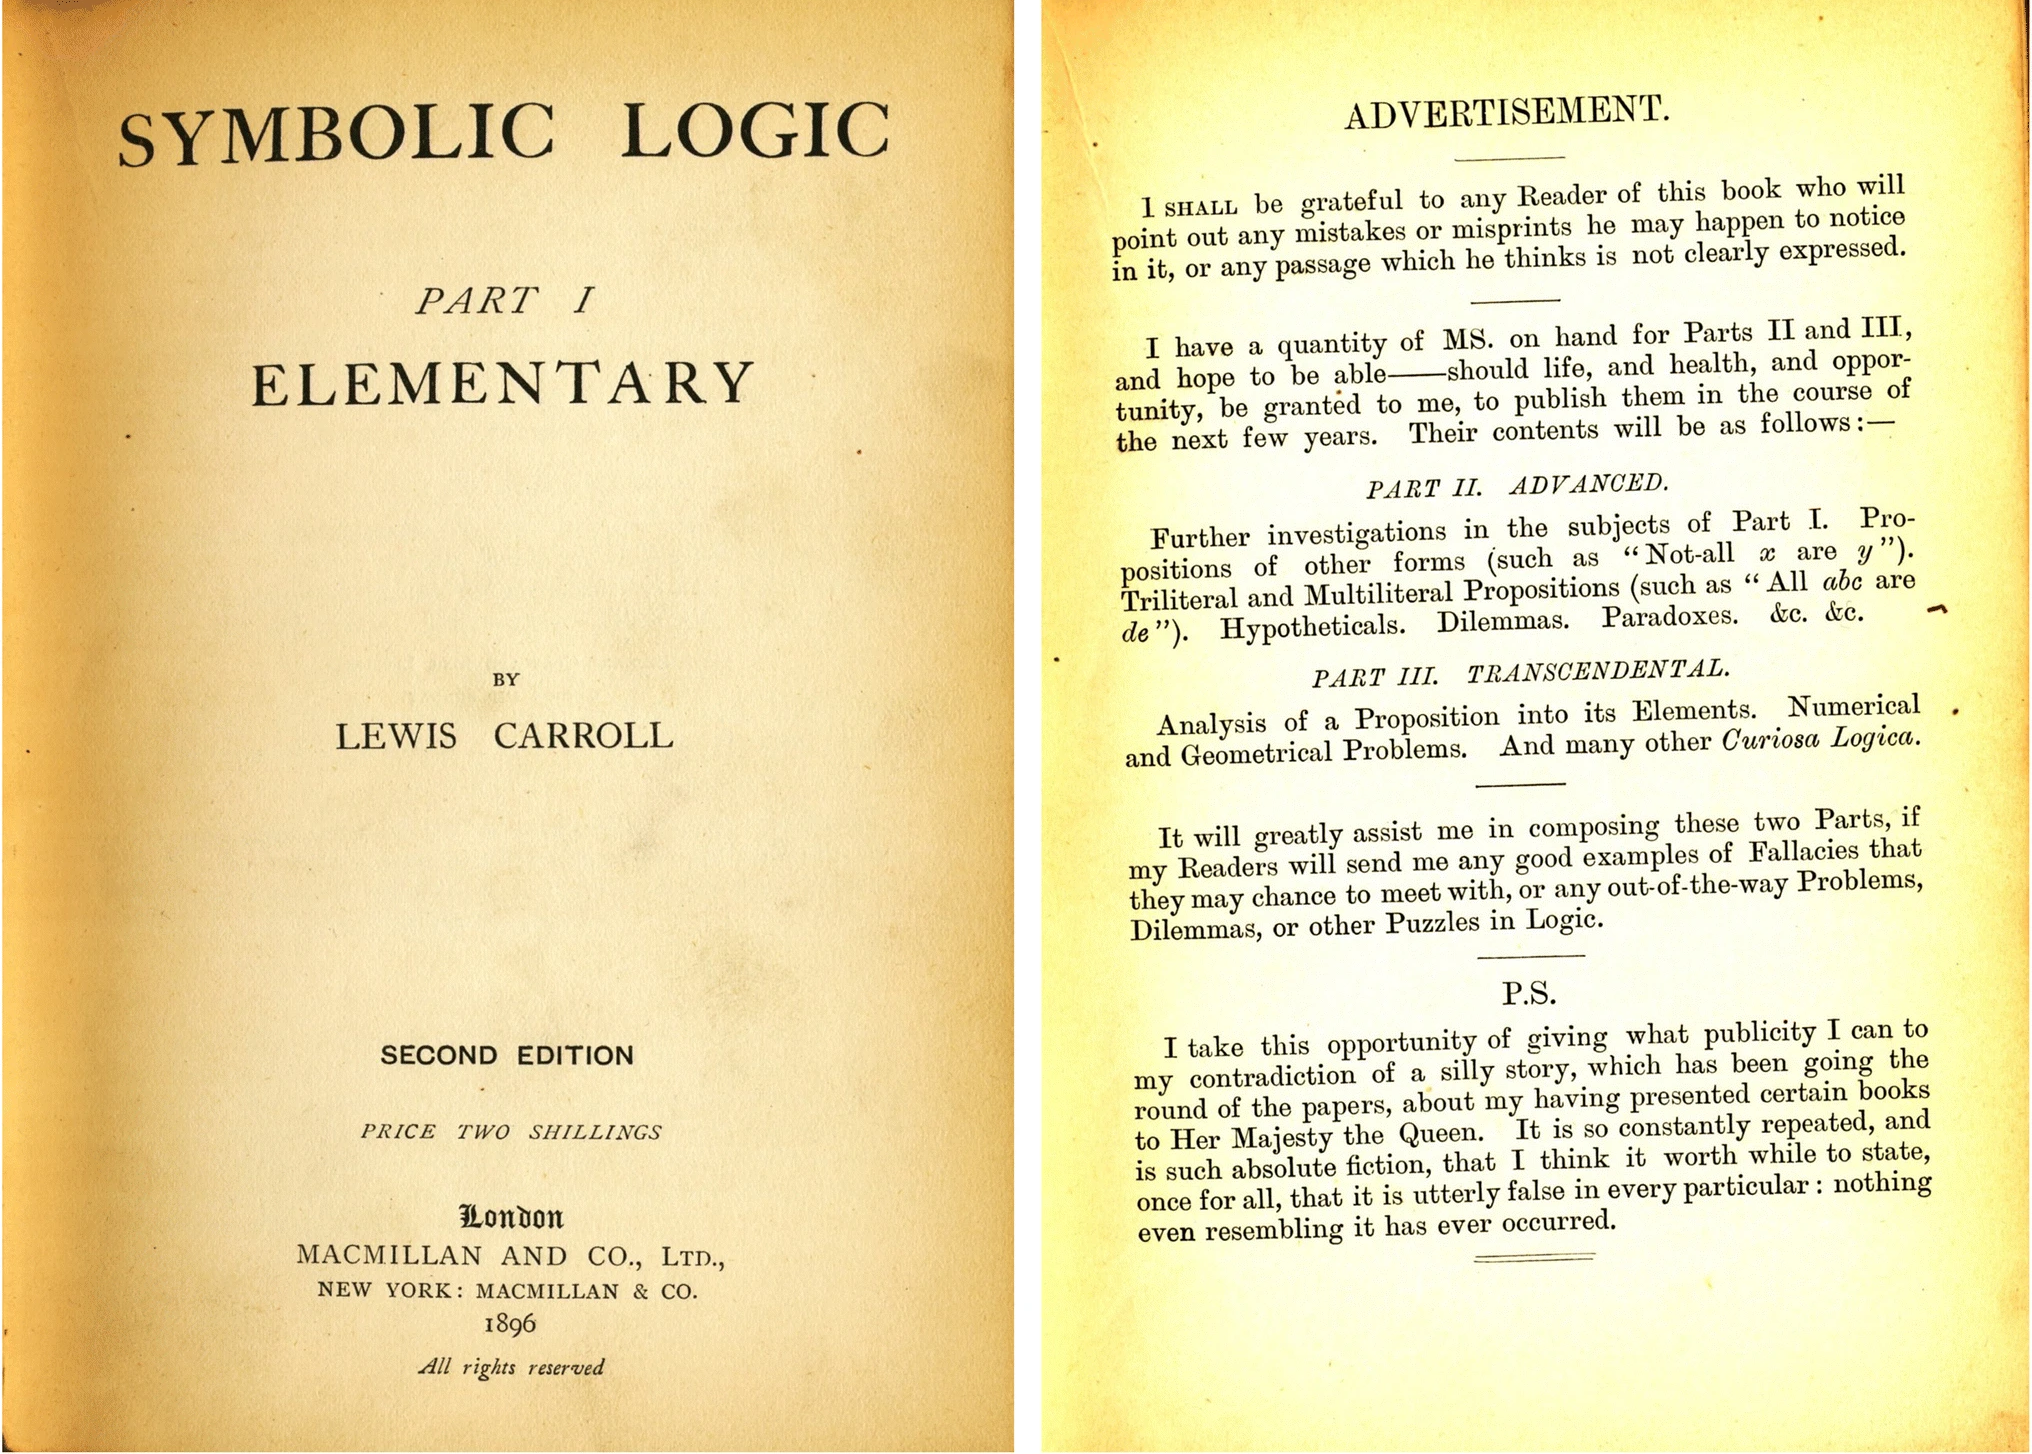
\includegraphics[width= 0.3\textwidth]{4}
				\caption{\small\textit{\color{gocco}Hình $4$.}}
				\vspace*{-5pt}
			\end{figure}
		\begin{figure}[H]
			\vspace*{5pt}
			\centering
			\captionsetup{labelformat= empty, justification=centering}
			\includegraphics[width= 0.3\textwidth]{5}
			\caption{\small\textit{\color{gocco}Hình $5$.}}
			\vspace*{-10pt}
		\end{figure}
		%	Đáp án tham khảo:
		%	-- $\pmb{1)}$	P$9-5$ P$5.6$\quad $\pmb{2)}$ Tg$6/1$ P$5/1$\quad $\pmb{3)}$ P$5.1$ P$5/1$\quad $\pmb{4)}$ P$5.1$ P$5/1$\quad $\pmb{5)}$ P$5.1$ P$5/1$\quad $\pmb{6)}$ P$5.1$ P$5/1$\quad $\pmb{7)}$ P$5.1$ P$5/1$\quad $\pmb{8)}$ P$5.1$ $(1-0)$
		%	\vskip 0.05cm
		%	-- $\\pmb{1)}$	C$6-5$ Tg$5-4$\quad $\pmb{2)}$ P$8-9$ T$3/1$\quad $\pmb{3)}$ P$9-2$ S$5/6$\quad $\pmb{4)}$ P$2.2$ S$6/5$\quad $\pmb{5)}$ C$5.1$ $(1-0)$
	\end{multicols}
\vspace*{-10pt}
\rule{1\textwidth}{0.1pt}
	\begin{center}
%		\vspace*{-5pt}
		\LARGE{\textbf{\color{gocco}LỜI GIẢI, ĐÁP ÁN}}
%		\vspace*{-5pt}
	\end{center}
	\begin{multicols}{2}
		\textbf{\color{gocco}Chuyến công tác đặc biệt}
		\vskip 0.05cm
		Sau mỗi giờ, đồng hồ của Xuân Phong chạy nhanh hơn đồng hồ của Lê Kính là $1+2= 3$ (phút). Vì vậy, thời gian để đồng hồ của Xuân Phong chạy nhanh hơn đồng hồ của Lê Kính $1$ tiếng $= 60$ (phút), là $60:3 = 20$ giờ. Thật là nguy hiểm cho một công tác quan trọng nếu không phát hiện ra lỗi của $2$ chiếc \linebreak đồng hồ.
		\vskip 0.05cm
		Để xác định các thám tử siêu việt đến từ đâu, các em hãy vẽ một vòng tròn tượng trưng cho chiếc bàn, xếp $3$ người theo thông tin ``\textit{Người đến từ TP. HCM ngồi giữa người đến từ Sa Đéc và người tên Vinh}" đặt cạnh\linebreak nhau (ngược hay thuận chiều kim không quan trọng, nên giả sử họ ngồi theo vị trí thuận chiều kim đồng hồ).
		\vskip 0.05cm
		Tiếp theo để ý tới thám tử có nhiều thông tin được thu nhập nhất, đó chính là thám tử Thu. Anh ta không thể sống ở Lào Cai, Phú Thọ (do trên bàn có $5$ người, và theo cách xếp, người ngồi cạnh Thu đối diện với người đến từ Phú Thọ), Gò Công lẫn Sa Đéc. Vì thế Thu đến từ TP. HCM. 
		\vskip 0.05cm
		Tiếp theo ``\textit{Người đến từ Lào Cai ngồi giữa Thu và Tố}", mà người ngồi bên tay phải của Thu đã đến từ Sa Đéc. Vì vậy ta biết được Vinh đến từ Lào Cai.
		\vskip 0.05cm
		Thông tin tiếp là ``\textit{Người đến từ Lào Cai \ldots\, đối diện anh ta là người đến từ Phú Thọ và Lê}". Ta đã biết đối diện với Vinh có $2$ người, trong đó một người đến từ Sa Đéc, vì thế, Lê là thám tử đến từ Sa Đéc.
		\vskip 0.05cm
		Còn hai vị trí còn lại dành cho Côn và Tố, và hai địa phương còn lại là Phú Thọ và Gò Công. Tuy nhiên do Tố ngồi cạnh Vinh, và một trong hai người ngồi đối diện với Vinh đến từ Phú Thọ, nên ta tìm ra ngay Côn đến từ Phú Thọ còn Tố đến từ Gò Công.
		\vskip 0.05cm
		Vậy các thám tử đã đến từ các vùng sau đây: \textit{Thu đến từ TP. HCM, Tố đến từ Gò Công, Lê đến từ Sa Đéc, Côn là người Phú Thọ còn Vinh đến từ Lào Cai.}
		\vskip 0.05cm
		\textbf{\color{gocco}Góc cờ}
		\vskip 0.05cm
		Đáp án tham khảo:
		\vskip 0.05cm
		-- $\pmb{1)}$	P$9-5$ P$5.6$\quad $\pmb{2)}$ Tg$6/1$ P$5/1$\quad $\pmb{3)}$ P$5.1$ P$5/1$\quad $\pmb{4)}$ P$5.1$ P$5/1$\quad $\pmb{5)}$ P$5.1$ P$5/1$\quad $\pmb{6)}$ P$5.1$ P$5/1$\quad $\pmb{7)}$ P$5.1$ P$5/1$\quad $\pmb{8)}$ P$5.1$ $(1-0)$
		\vskip 0.05cm
		-- $\pmb{1)}$	C$6-5$ Tg$5-4$\quad $\pmb{2)}$ P$8-9$ T$3/1$\quad $\pmb{3)}$ P$9-2$ S$5/6$\quad $\pmb{4)}$ P$2.2$ S$6/5$\quad $\pmb{5)}$ C$5.1$ $(1-0)$
\end{multicols}
	
	
	
	
	
	
